\section{PaaS}
Platform as a Service is a cloud computing model that provides developers with a platform for building, running and managing applications, it allows developers to focus on creating their applications without having to worry about infrastructure management. \n
A couple of very relevant examples are:
\begin{itemize}
    \item Github
    \item Java, Python, Go, etc...
\end{itemize}
Common Platforms allow the deployment of web applications, a couple of examples could be:
\begin{itemize}
    \item Netlify, which only allows free deployment and management of a web application.
    \item Google App Engine, allows development, deployment and management of web applications. It also offers automatic scaling, high availability and load balancing for applications.
\end{itemize}
\subsection{Heroku}
Heroku, just like Netlify, allows deployment of web applications via Github integration, this idea allows for easy updates to the application. \n
Heroku can scale horizontally or vertically, this allows for easy handling of fluctuations in traffic and ensures that the applciation is always available. It also provides many add-ons to ease application management. \n
Dynos are lightweight containers (similar to Docker's) that run and manage applications. They are used to provide horizontal scaling and ensure that the appliction is always available. Everything can be controlled via CLI, just like with Kubernetes.
\subsection{Google App Engine}
Google App Engine supports multiple programming languages and is able to scale the application automatically depending on traffic and usage patterns, developers do not have to manually adjust resources, and can rely on the platform to automatically handle traffic spikes. \n
Since the service is offered from Google the client can expect high availability and reliability, plus a tight interaction with other Google cloud services. \n
Google App Engine provides a range of development and deployment tools. \n
The service also provides a series of predetermined classes (instance classes) that developers can choose from based on their application's requirements.
\subsection{AWS Elastic Beanstalk}
Elastic Beanstalk is just the AWS version of Google App Engine, with minor differences like the automatic environment set up, which basically provides the client an environment built around the web application automatically. For the rest is just a different name for the same topping we have seen for Google's solution.
\subsection{AWS Lambda}
AWS Lambda is a serverless computing service provided by Amazon, it can be used for a variety of fields like: web applications, data processing and IoT applications. It can, of course, be integrated with a wide variety of other AWS services. \n
Serverless functions are event-driven, which means that they are triggered by events such as HTTP requests, database updates or messages from a message queue. When an event triggers a serverless function:
\begin{itemize}
    \item The cloud provider creates a new instance of the function and runs it in a containerized environment.
    \item The function code is then exectured.
    \item The result is returned to the caller.
\end{itemize}
\subsection{Vercel}
Vercel is a platform for deploying and hosting static websites and serverless functions.
\subsection{Cloud foundry}
Cloud Foundry is an open-PaaS solution capable of supporting any language or framework, it was originally developed by VMware and later became a stand-alone company. It can interact with most cloud providers and allows customers to:
\begin{itemize}
    \item Transfer applications to other cloud providers.
    \item Transfer between public and private clouds without having to make changes to the application.
\end{itemize}
What allows Cloud Foundry to be so pervasive is the concept of buildpack. \n
A buildpack is a set of executables that inspects the provided source code and creates a plan to build and run the application. A typical buildpack consists of the following files:
\begin{itemize}
    \item \textsf{buildpack.toml} - provides metadata about the buildpack
    \item \textsf{bin/detect} - determines wether the buildpack should be applied
    \item \textsf{bin/build} - executes the build logic
\end{itemize}
When an application is uploaded to Cloud Foundry the buildpack to be used for proper operation of the application is indicated, the service identifies the buildpack to be used an installs it in the Droplet Execution Agent, where the application runs. \n
The environment is customized via what the client specifies, the logic is similar to the use of images taken from Dockerhub when doing a compose. \n
Cloud Foundry has a modular architecture that consists of several components, including the Cloud Controller (which manages the deployment of applications and services), Routing Component (which handles the traffic between the application and external services), Loggregator (which is just a centralized logging system) and Diego (which is responsible for managing application instances). The architecture can be seen in detail in figure 11.
\begin{figure}
    \centering
    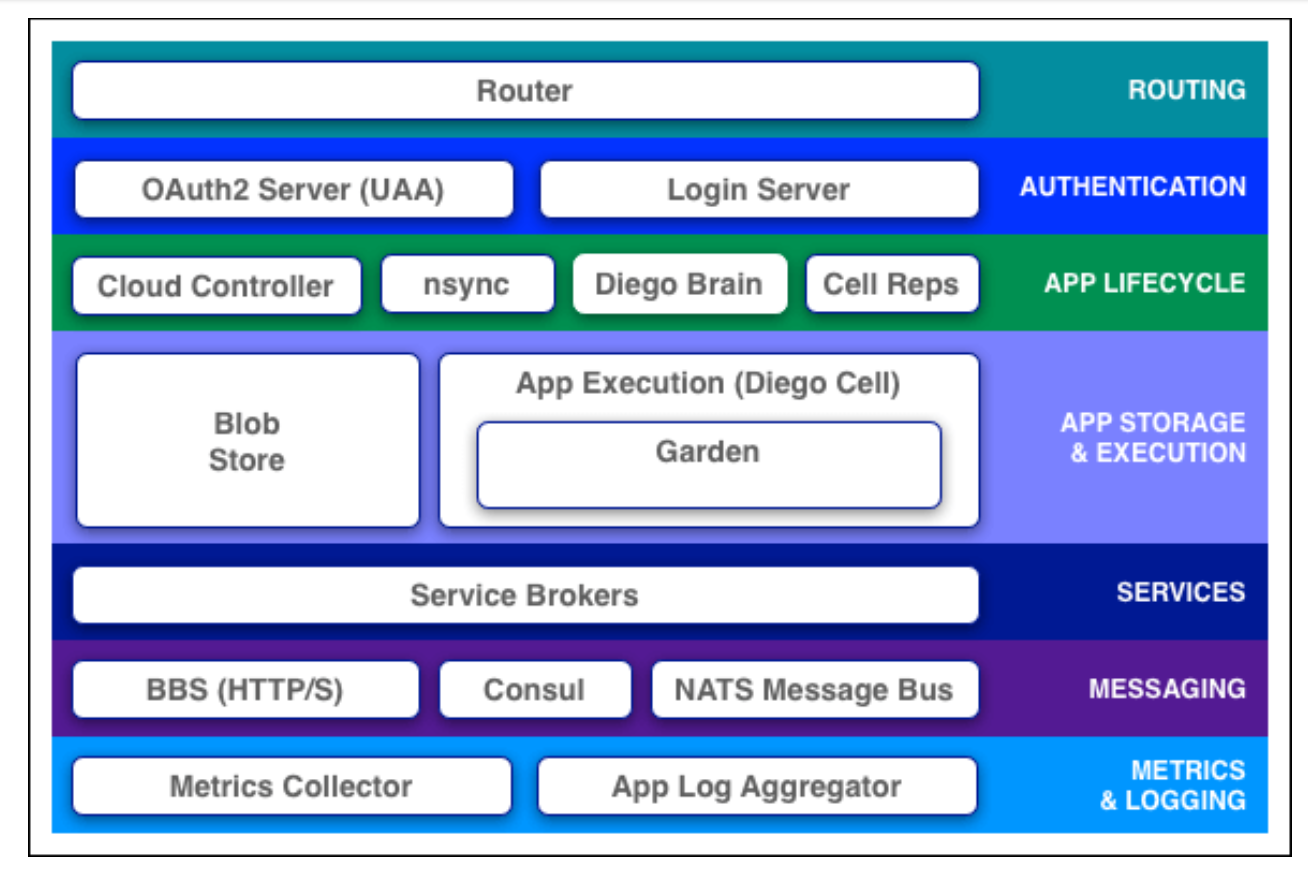
\includegraphics[scale=0.5]{./Images/Cloud_Foundry.png}
    \caption{Cloud Foundry's architecture}
\end{figure}
Now we will go through the various levels:
\subsubsection{Routing}
The router routes incoming traffic to the appropriate component, either a Cloud Controller component or a hosted application running on a Diego Cell, the router periodically queries the Diego Bulletin Board System to determine which cells and containers each application currently runs on. Using these informations the router recomputes new routing tables based on the IP addresses of each cell virtual machine.
\subsubsection{Authentication}
The Authentication contains an OAuth server and a login server, the servers work together to provide identity management.
\subsubsection{App lifecycle}
The app lifecycle layer contains the Cloud Controller and Diego Brain. The controller directs the deployment of applications and support push operation of an app to Cloud Foundry, it also directs the diego brain through the cc-bridge components to coordinate individual Diego cells to stage and run applications. \n
nsync, BBS and Cell reps work together along a chain to keep apps running. At one end is the user, at the other end are the instances of applications running on widely distributed VMs. In particular:
\begin{itemize}
    \item Nsync - recieves a message from the cloud controller when the user scales an app.
    \item BBS - uses its convergence process to monitor the DesiredLRP and ActualLRP values.
    \item Cell rep - monitors the containers and provides the ActualLRP value.
\end{itemize}
\subsubsection{AppStorage and Execution}
In this layer we find the Blob store, which is a repository for large binary files, which Github cannot easily manage, because Github is made for code. The Blob store contains the following:
\begin{itemize}
    \item Application code packages
    \item Buildpacks
    \item Droplets
\end{itemize}
It can be configured as an internal server or an external s3 endpoint. \n
Here we also find the heart of the execution, the Diego Cell.
\subsubsection{Services}
Here resides the Service Broker, which basically provisions and binds needed services to applications.
\subsubsection{Messaging}
The internal communication is handled through HTTP / HTTPS / BBS, where BBS is Diego's Bulletin Board System. The BBS stores more frequently updated and disposable data such as cell and app status, unallocated work and heartbeat messages, as well as longer-lived distributed locks.
\subsubsection{Metrics and Logging}
Last but not least we have th metrics and logging systems which consists of a Metrics Collector that shoves everything into the Loggregator that crunches through stuff and writes logs. \n
Communication is handled through the NATS bus which is lightweight and its messaging is based on the publish-subscribe model.